% ----------------------------------------------------------------------------
% File: CentreNautique.tex
% Usage: Latex2e
% Creation :  21 janv 2022 sergemorvan29@gmail.com
% Revised:   
% Revised:   
% ----------------------------------------------------------------------------
\documentclass[12pt, report]{article}
% ----------------------------------------------------------------------------
%-------------------------------------------------------------------------
\usepackage{helvet}
\usepackage[utf8]{inputenc}
\usepackage[french]{babel}
\usepackage{moreverb}
\usepackage{eurosym}
\usepackage{textcomp}
\usepackage{index}
\usepackage{amsfonts}
\usepackage{graphics}
\usepackage{listings}
\usepackage{hyperref}
\usepackage{multimedia}
\usepackage{pgfpages}
\usepackage{pgf,xcolor,tikz}
\usepackage{rotating}
\usepackage{framed}
\usepackage[framed,hyperref,standard]{ntheorem}
\usepackage{fancyhdr,lastpage}
\usepackage{fancyvrb}
\usepackage{geometry}
\geometry{margin=40pt}
\begin{document}
\begin{center}
\begin{minipage}{16cm}

\begin{center}
{\sc\bf\LARGE Activités maritimes  en Rade de Brest. }\\
\vspace{2cm}
Auteur : Terre Virtuelle \hfill 3/31/2022

\end{center}
\end{minipage}
\end{center}

\vspace{2cm}
%%%%%%%%%%%%%%%%%%%%%%%%%%%%%%%%%%%%%%%%%%%%%%%%%%%%%%%%%%%%%%%%%
\section*{Introduction} 

\section{Question}
Départ : Vous êtes au port du Moulin Blanc.  De quel type de port s’agit-il ?
\subsection*{Réponse}
C'est un port de Plaisance ou une Marina.
%%%%%%%%%%%%%%%%%%%%%%%%%%%%%%%%%%%%%%%%%%%%%%%%%%%%%%%%%%%%%%%%%%%%%%%
\begin{center}
\framebox[1\width]{
	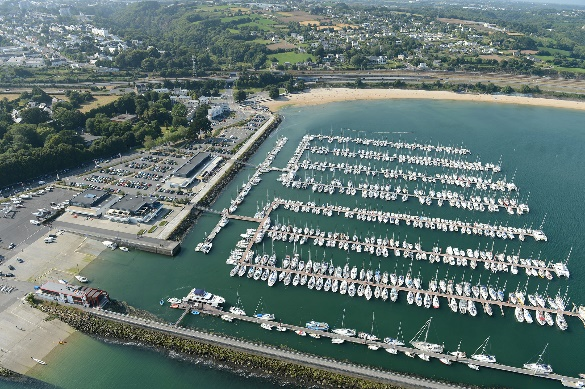
\includegraphics[ width=10cm]{data/scenarios/scenarioCN/images/img1.png}
}
\begin{figure}[ht]
\caption{\textit{Marina du Moulin Blanc}}
\end{figure}
\end{center}
%%%%%%%%%%%%%%%%%%%%%%%%%%%%%%%%%%%%%%%%%%%%%%%%%%%%%%%%%%%%%%%%%%%%%%%

\section{Question}
J’ai une petite faim. Je connais un bon ostréiculteur. Cap au 130 et rendez-vous sur la cale. Comment se nomme le lieu où je vais accoster?
\subsection*{Réponse}
C'est le port de Kéraliou

\section{Question}
Que produit un ostréiculteur ?
\subsection*{Réponse}
Un ostréicuteur élève des huîtres.
%%%%%%%%%%%%%%%%%%%%%%%%%%%%%%%%%%%%%%%%%%%%%%%%%%%%%%%%%%%%%%%%%%%%%%%
\begin{center}
\framebox[1\width]{
	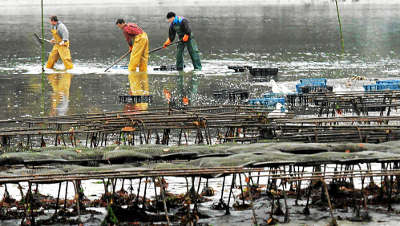
\includegraphics[ width=10cm]{data/scenarios/scenarioCN/images/img2.png}
}
\begin{figure}[ht]
\caption{\textit{Les poches à huîtres}}
\end{figure}
\end{center}
%%%%%%%%%%%%%%%%%%%%%%%%%%%%%%%%%%%%%%%%%%%%%%%%%%%%%%%%%%%%%%%%%%%%%%%
%%%%%%%%%%%%%%%%%%%%%%%%%%%%%%%%%%%%%%%%%%%%%%%%%%%%%%%%%%%%%%%%%%%%%%%
\begin{center}
\framebox[1\width]{
	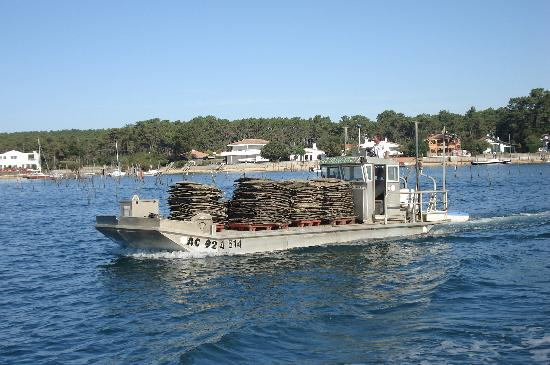
\includegraphics[ width=10cm]{data/scenarios/scenarioCN/images/img3.png}
}
\begin{figure}[ht]
\caption{\textit{Une barge}}
\end{figure}
\end{center}
%%%%%%%%%%%%%%%%%%%%%%%%%%%%%%%%%%%%%%%%%%%%%%%%%%%%%%%%%%%%%%%%%%%%%%%

\section{Question}
J’aperçois, au cap 265,  presque plein Ouest, un gros bateau qui décharge sa cargaison. J’y ferais bien un tour. De quel lieu s'agit-il ?
\subsection*{Réponse}
C'est le port de commerce
%%%%%%%%%%%%%%%%%%%%%%%%%%%%%%%%%%%%%%%%%%%%%%%%%%%%%%%%%%%%%%%%%%%%%%%
\begin{center}
\framebox[1\width]{
	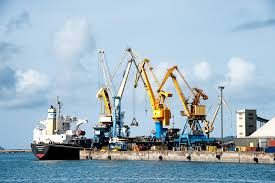
\includegraphics[ width=10cm]{data/scenarios/scenarioCN/images/img4.png}
}
\begin{figure}[ht]
\caption{\textit{Grues}}
\end{figure}
\end{center}
%%%%%%%%%%%%%%%%%%%%%%%%%%%%%%%%%%%%%%%%%%%%%%%%%%%%%%%%%%%%%%%%%%%%%%%

\section{Question}
Que peuvent décharger ces gros bateaux ?
\subsection*{Réponse}
Dans un port de commerce on décharge toute sorte de matières. Du pétrole, du gaz, du blé,  des containers. Regardes!  c'est le Queen Marie 2, en réparation.
%%%%%%%%%%%%%%%%%%%%%%%%%%%%%%%%%%%%%%%%%%%%%%%%%%%%%%%%%%%%%%%%%%%%%%%
\begin{center}
\framebox[1\width]{
	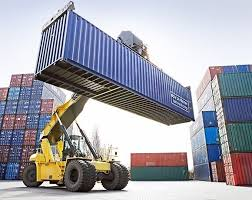
\includegraphics[ width=10cm]{data/scenarios/scenarioCN/images/img5.png}
}
\begin{figure}[ht]
\caption{\textit{Containers}}
\end{figure}
\end{center}
%%%%%%%%%%%%%%%%%%%%%%%%%%%%%%%%%%%%%%%%%%%%%%%%%%%%%%%%%%%%%%%%%%%%%%%

\section{Question}
Mon ami Loïc m’a donné rendez-vous à bord de son coquillier pour une partie de pêche ! Cap au 175. Il m’attend au Banc du Corbeau. Que pêche Loïc ?
\subsection*{Réponse}
Il pêche la coquilles Saint Jacques. En latin : Pecten maximus.
%%%%%%%%%%%%%%%%%%%%%%%%%%%%%%%%%%%%%%%%%%%%%%%%%%%%%%%%%%%%%%%%%%%%%%%
\begin{center}
\framebox[1\width]{
	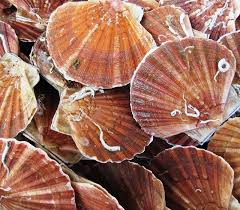
\includegraphics[ width=10cm]{data/scenarios/scenarioCN/images/img6.png}
}
\begin{figure}[ht]
\caption{\textit{Coquilles Saint Jacques}}
\end{figure}
\end{center}
%%%%%%%%%%%%%%%%%%%%%%%%%%%%%%%%%%%%%%%%%%%%%%%%%%%%%%%%%%%%%%%%%%%%%%%
%%%%%%%%%%%%%%%%%%%%%%%%%%%%%%%%%%%%%%%%%%%%%%%%%%%%%%%%%%%%%%%%%%%%%%%
\begin{center}
\framebox[1\width]{
	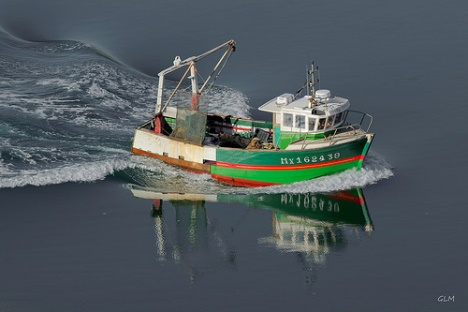
\includegraphics[ width=10cm]{data/scenarios/scenarioCN/images/img7.png}
}
\begin{figure}[ht]
\caption{\textit{Coquillier en pêche}}
\end{figure}
\end{center}
%%%%%%%%%%%%%%%%%%%%%%%%%%%%%%%%%%%%%%%%%%%%%%%%%%%%%%%%%%%%%%%%%%%%%%%
%%%%%%%%%%%%%%%%%%%%%%%%%%%%%%%%%%%%%%%%%%%%%%%%%%%%%%%%%%%%%%%%%%%%%%%
\begin{center}
\framebox[1\width]{
	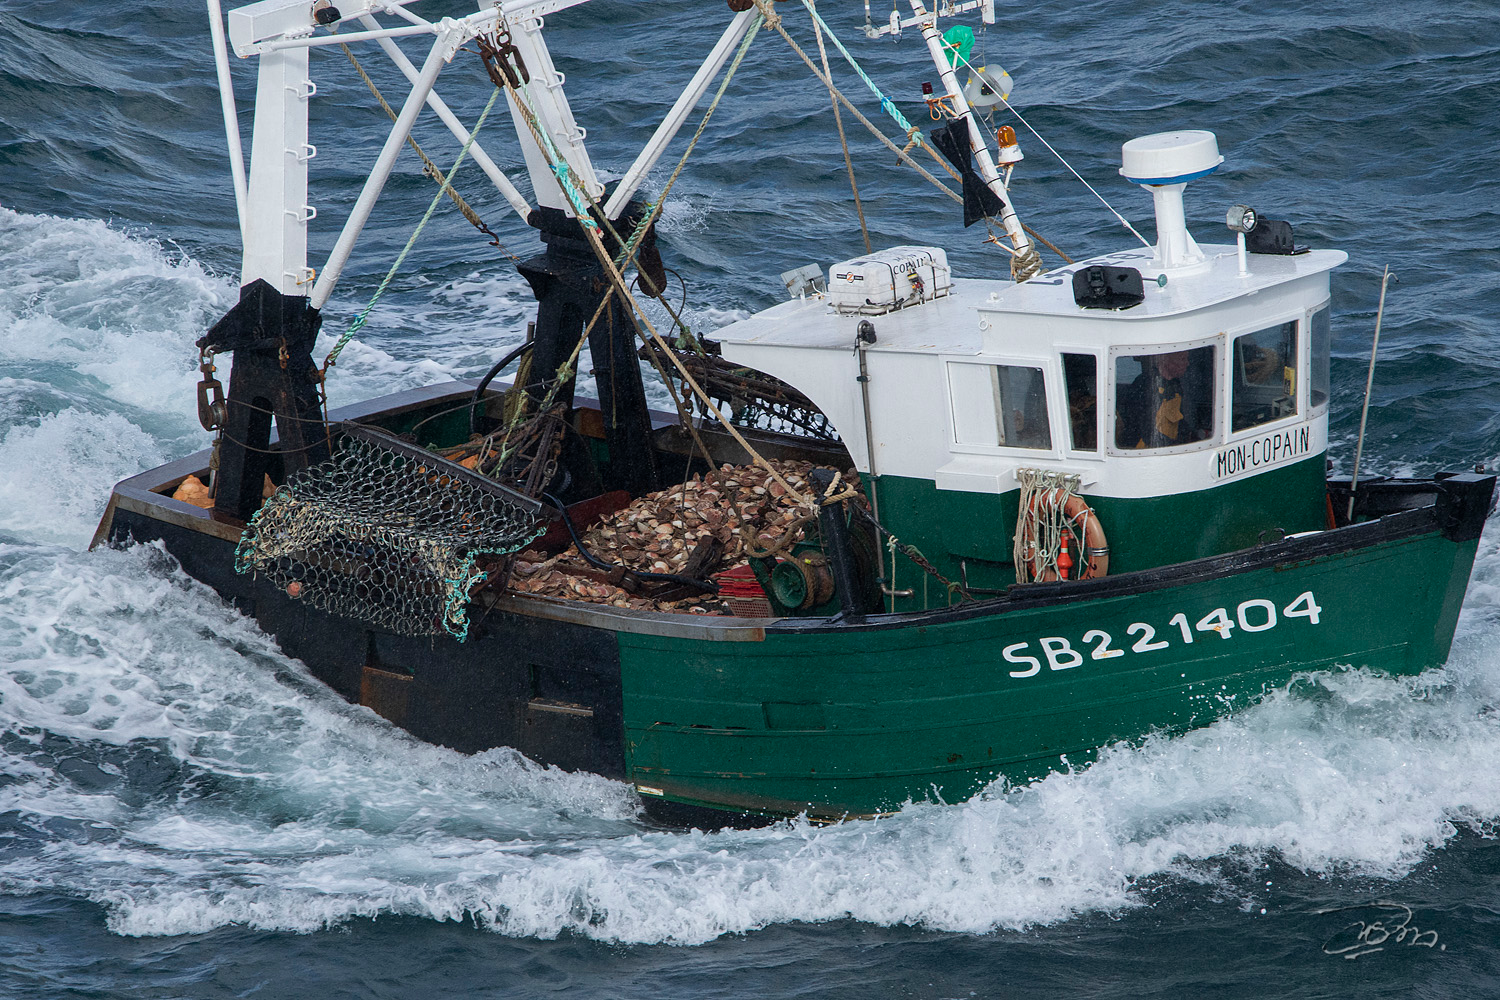
\includegraphics[ width=10cm]{data/scenarios/scenarioCN/images/img8.png}
}
\begin{figure}[ht]
\caption{\textit{Coquillier en pêche}}
\end{figure}
\end{center}
%%%%%%%%%%%%%%%%%%%%%%%%%%%%%%%%%%%%%%%%%%%%%%%%%%%%%%%%%%%%%%%%%%%%%%%

\section{Question}
Nous décidons de poursuivre notre cap au 175 pour déguster notre pêche à l’abri d’une île.  Question : De quel îlot, situé à 400 mètres au Sud-Ouest de la Pointe de l'Armorique s’agit-il ?
\subsection*{Réponse}
C'est l'Ile Ronde.
%%%%%%%%%%%%%%%%%%%%%%%%%%%%%%%%%%%%%%%%%%%%%%%%%%%%%%%%%%%%%%%%%%%%%%%
\begin{center}
\framebox[1\width]{
	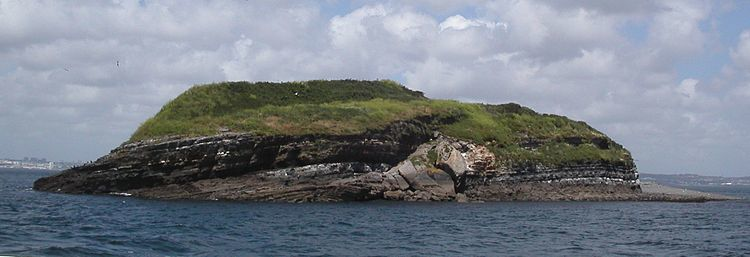
\includegraphics[ width=10cm]{data/scenarios/scenarioCN/images/img9.png}
}
\begin{figure}[ht]
\caption{\textit{L'Ile Ronde}}
\end{figure}
\end{center}
%%%%%%%%%%%%%%%%%%%%%%%%%%%%%%%%%%%%%%%%%%%%%%%%%%%%%%%%%%%%%%%%%%%%%%%

\section{Question}
 Pendant notre repas, Paul me raconte un fait marquant de la seconde guerre mondiale. En mer, à 600 m à l’est de l’Île Ronde, se trouvent deux gros cubes en béton construits par l’occupant lors de la seconde Guerre mondiale. Ils avaient vocation à accueillir le cuirassé Bismarck de la Kriegsmarine. Les deux cubes ont pour cela été installés à un endroit où la profondeur est de 16 mètres. Mais, coulé avant d'avoir pu atteindre la rade de Brest, le cuirassé n’a jamais utilisé ces cubes de béton. De quoi me parle-t-il ? Recherchez-les sur une carte.
\subsection*{Réponse}
Ce sont les Ducs D'Albe
%%%%%%%%%%%%%%%%%%%%%%%%%%%%%%%%%%%%%%%%%%%%%%%%%%%%%%%%%%%%%%%%%%%%%%%
\begin{center}
\framebox[1\width]{
	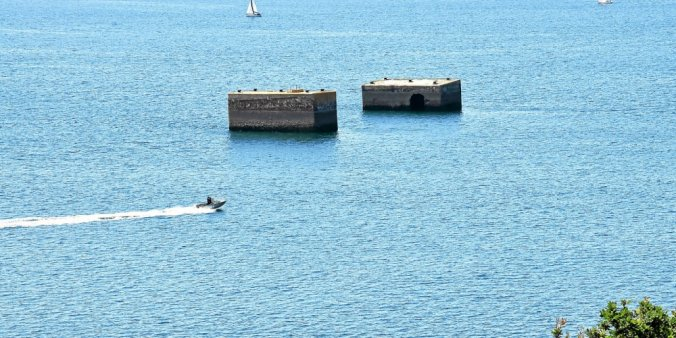
\includegraphics[ width=10cm]{data/scenarios/scenarioCN/images/img10.png}
}
\begin{figure}[ht]
\caption{\textit{Les ducs d'Albe}}
\end{figure}
\end{center}
%%%%%%%%%%%%%%%%%%%%%%%%%%%%%%%%%%%%%%%%%%%%%%%%%%%%%%%%%%%%%%%%%%%%%%%

\section{Question}
Loïc me propose de rejoindre son ami Gaël spécialisé dans la mytiliculture. Cap au 100 et rendez-vous sur le lieu d’exploitation, au niveau du banc du Caplan. En quoi consiste le métier du mytiliculteur ? 
\subsection*{Réponse}
La mytiliculture désigne l'élevage des moules. En latin : Mytilus edulis. En Bretagne on trouve essentiellement des élevages  sur bouchots ou sur des filières.
%%%%%%%%%%%%%%%%%%%%%%%%%%%%%%%%%%%%%%%%%%%%%%%%%%%%%%%%%%%%%%%%%%%%%%%
\begin{center}
\framebox[1\width]{
	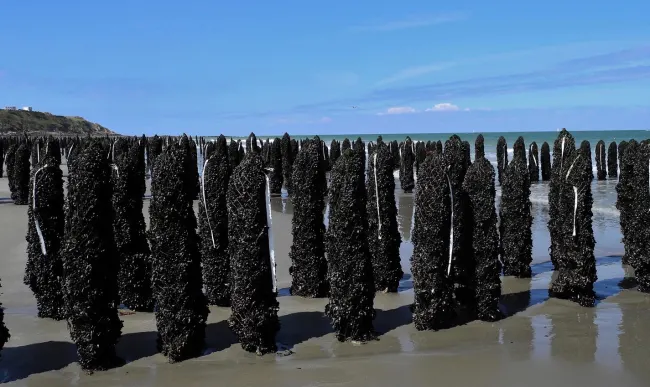
\includegraphics[ width=10cm]{data/scenarios/scenarioCN/images/img11.png}
}
\begin{figure}[ht]
\caption{\textit{Elevage sur bouchots}}
\end{figure}
\end{center}
%%%%%%%%%%%%%%%%%%%%%%%%%%%%%%%%%%%%%%%%%%%%%%%%%%%%%%%%%%%%%%%%%%%%%%%
%%%%%%%%%%%%%%%%%%%%%%%%%%%%%%%%%%%%%%%%%%%%%%%%%%%%%%%%%%%%%%%%%%%%%%%
\begin{center}
\framebox[1\width]{
	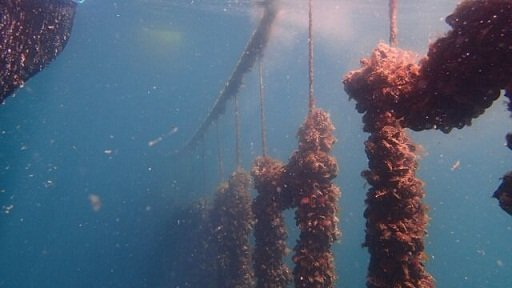
\includegraphics[ width=10cm]{data/scenarios/scenarioCN/images/img12.png}
}
\begin{figure}[ht]
\caption{\textit{Elevage sur corde}}
\end{figure}
\end{center}
%%%%%%%%%%%%%%%%%%%%%%%%%%%%%%%%%%%%%%%%%%%%%%%%%%%%%%%%%%%%%%%%%%%%%%%

\section{Question}
Après avoir découvert le métier de Gaël, je décide de poursuivre ma route maritime vers l'ouest, cap au 270.  Je me dirige vers une zone militaire ultra protégée , interdite au public.  Des hommes armés guettent l’ennemi du haut des miradors. Ce lieu abrite des navires capables de se déplacer en surface et sous l’eau. Comment se nomme ce lieu très surveillé ? 
\subsection*{Réponse}
C'est l'Ile Longue. Commencés en 1967, les travaux ont durés cinq ans.

\section{Question}
Qui y travaillent ?
\subsection*{Réponse}
Des militaires et des civils habilités.

\section{Question}
Que cache de particulier cet endroit ? 
\subsection*{Réponse}
Des sous-marins nucléaires.
%%%%%%%%%%%%%%%%%%%%%%%%%%%%%%%%%%%%%%%%%%%%%%%%%%%%%%%%%%%%%%%%%%%%%%%
\begin{center}
\framebox[1\width]{
	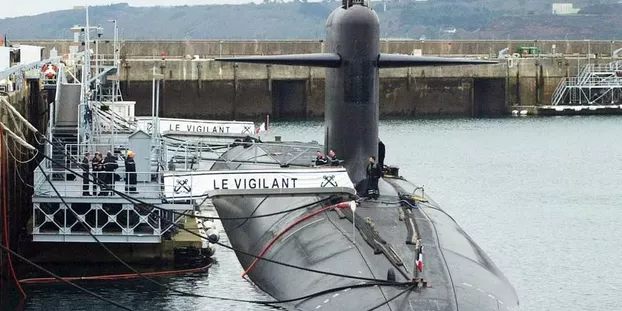
\includegraphics[ width=10cm]{data/scenarios/scenarioCN/images/img13.png}
}
\begin{figure}[ht]
\caption{\textit{Sous-marin nucléaire}}
\end{figure}
\end{center}
%%%%%%%%%%%%%%%%%%%%%%%%%%%%%%%%%%%%%%%%%%%%%%%%%%%%%%%%%%%%%%%%%%%%%%%

\section{Question}
N’ayant pas la possibilité d’accoster sur cette partie de la côte, je décide de poursuivre ma visite de la Rade. Cap au 355. Sur mon chemin, je croise un fileyeur. Je fais bien attention de m’écarter pour ne pas le déranger dans son activité. Quelle est l’activité du fileyeur ?
\subsection*{Réponse}
Le fileyeur est un bateau de pêche qui utilise plusieurs types de filets, tels que le trémail ou le filet droit. 
%%%%%%%%%%%%%%%%%%%%%%%%%%%%%%%%%%%%%%%%%%%%%%%%%%%%%%%%%%%%%%%%%%%%%%%
\begin{center}
\framebox[1\width]{
	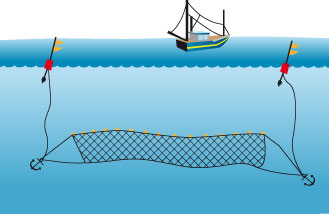
\includegraphics[ width=10cm]{data/scenarios/scenarioCN/images/img14.png}
}
\begin{figure}[ht]
\caption{\textit{Filet}}
\end{figure}
\end{center}
%%%%%%%%%%%%%%%%%%%%%%%%%%%%%%%%%%%%%%%%%%%%%%%%%%%%%%%%%%%%%%%%%%%%%%%
%%%%%%%%%%%%%%%%%%%%%%%%%%%%%%%%%%%%%%%%%%%%%%%%%%%%%%%%%%%%%%%%%%%%%%%
\begin{center}
\framebox[1\width]{
	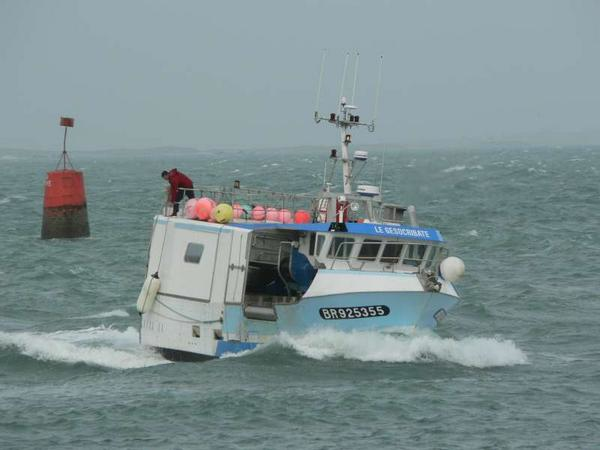
\includegraphics[ width=10cm]{data/scenarios/scenarioCN/images/img15.png}
}
\begin{figure}[ht]
\caption{\textit{Fileyeur}}
\end{figure}
\end{center}
%%%%%%%%%%%%%%%%%%%%%%%%%%%%%%%%%%%%%%%%%%%%%%%%%%%%%%%%%%%%%%%%%%%%%%%
%%%%%%%%%%%%%%%%%%%%%%%%%%%%%%%%%%%%%%%%%%%%%%%%%%%%%%%%%%%%%%%%%%%%%%%
\begin{center}
\framebox[1\width]{
	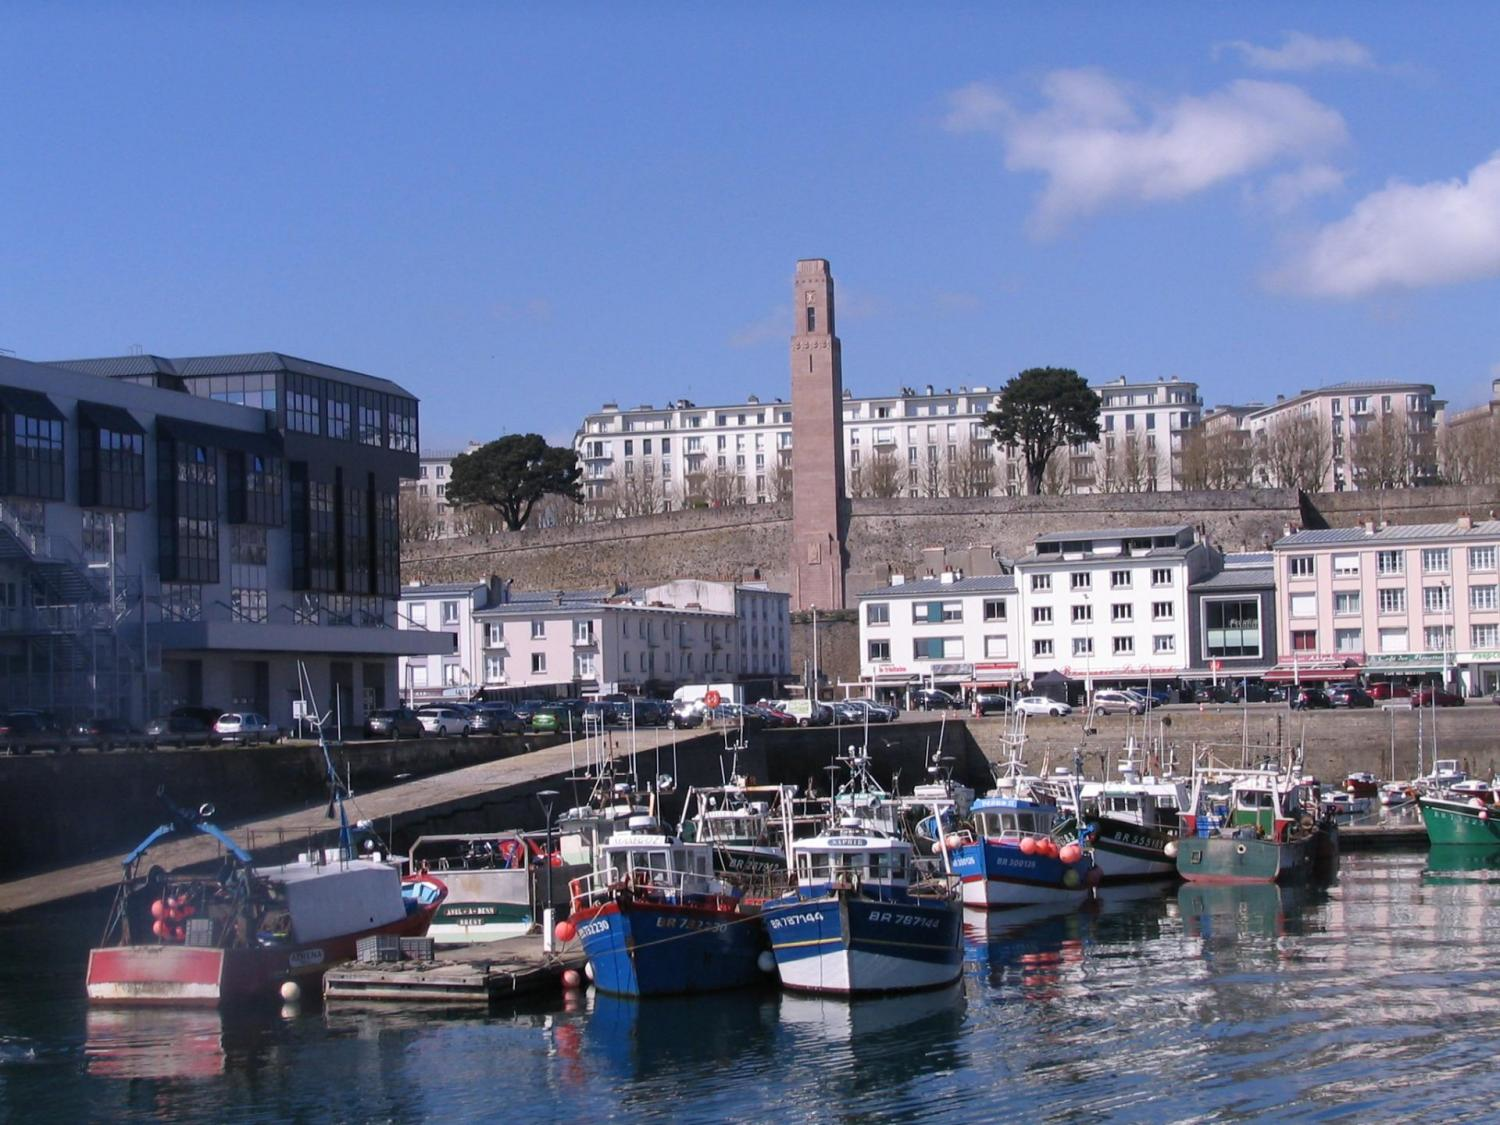
\includegraphics[ width=10cm]{data/scenarios/scenarioCN/images/img16.png}
}
\begin{figure}[ht]
\caption{\textit{Fileyeurs à Brest}}
\end{figure}
\end{center}
%%%%%%%%%%%%%%%%%%%%%%%%%%%%%%%%%%%%%%%%%%%%%%%%%%%%%%%%%%%%%%%%%%%%%%%

\section{Question}
En poursuivant ma route, je prends le soin de laisser la bouée de chenal « Penoupell » à bâbord. Mon nouveau cap est au 15. Vite ! Le commandant Rousseau m’a invité au baptême du nouveau vaisseau de guerre basé dans les bassins de l’Arsenal, je ne dois pas être en retard ! Retrouvez les images qui correspondent à cette activité et son lieu maritime.
\subsection*{Réponse}
Le port militaire
%%%%%%%%%%%%%%%%%%%%%%%%%%%%%%%%%%%%%%%%%%%%%%%%%%%%%%%%%%%%%%%%%%%%%%%
\begin{center}
\framebox[1\width]{
	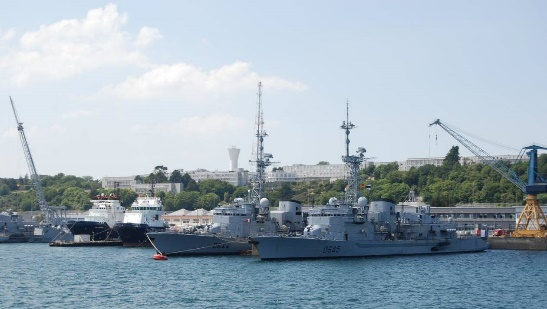
\includegraphics[ width=10cm]{data/scenarios/scenarioCN/images/img17.png}
}
\begin{figure}[ht]
\caption{\textit{Le port militaire}}
\end{figure}
\end{center}
%%%%%%%%%%%%%%%%%%%%%%%%%%%%%%%%%%%%%%%%%%%%%%%%%%%%%%%%%%%%%%%%%%%%%%%
%%%%%%%%%%%%%%%%%%%%%%%%%%%%%%%%%%%%%%%%%%%%%%%%%%%%%%%%%%%%%%%%%%%%%%%
\begin{center}
\framebox[1\width]{
	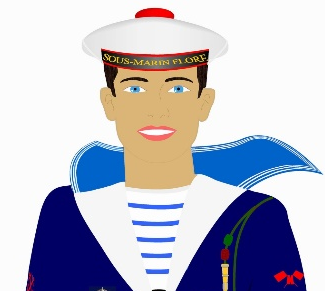
\includegraphics[ width=10cm]{data/scenarios/scenarioCN/images/img18.png}
}
\begin{figure}[ht]
\caption{\textit{Un marin de la marine nationale}}
\end{figure}
\end{center}
%%%%%%%%%%%%%%%%%%%%%%%%%%%%%%%%%%%%%%%%%%%%%%%%%%%%%%%%%%%%%%%%%%%%%%%

\section{Question}
Il est déjà l’heure de rentrer au port. Cap au 75. Sur le chemin du retour, je croise un caseyeur qui lui aussi rentre à terre. Qu’elle est l’activité du caseyeur ? 
\subsection*{Réponse}
Un caseyeur est un bateau de pêche utilisant des casiers destinés à la pêche aux tourteaux, aux araignées, aux homards et aux étrilles.
%%%%%%%%%%%%%%%%%%%%%%%%%%%%%%%%%%%%%%%%%%%%%%%%%%%%%%%%%%%%%%%%%%%%%%%
\begin{center}
\framebox[1\width]{
	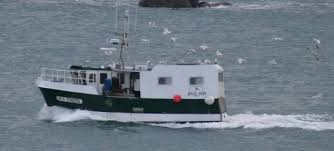
\includegraphics[ width=10cm]{data/scenarios/scenarioCN/images/img19.png}
}
\begin{figure}[ht]
\caption{\textit{Caseyeur}}
\end{figure}
\end{center}
%%%%%%%%%%%%%%%%%%%%%%%%%%%%%%%%%%%%%%%%%%%%%%%%%%%%%%%%%%%%%%%%%%%%%%%

\section{Question}
Que trouve-t-on dans  sur son pont ou dans ses cales ?
\subsection*{Réponse}
Des casiers
%%%%%%%%%%%%%%%%%%%%%%%%%%%%%%%%%%%%%%%%%%%%%%%%%%%%%%%%%%%%%%%%%%%%%%%
\begin{center}
\framebox[1\width]{
	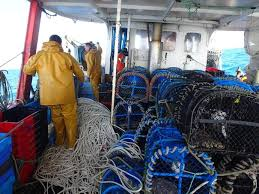
\includegraphics[ width=10cm]{data/scenarios/scenarioCN/images/img20.png}
}
\begin{figure}[ht]
\caption{\textit{}}
\end{figure}
\end{center}
%%%%%%%%%%%%%%%%%%%%%%%%%%%%%%%%%%%%%%%%%%%%%%%%%%%%%%%%%%%%%%%%%%%%%%%

\section{Question}

\subsection*{Réponse}

\end{document}